\documentclass[12pt]{article}
% \usepackage[top=1in,left=1in, right = 1in, footskip=1in]{geometry}
\usepackage[top=1in,footskip=1in]{geometry}

\usepackage{graphicx}
\usepackage{xspace}
%\usepackage{adjustbox}

\usepackage{multirow}
\usepackage{booktabs}

\usepackage{pdflscape}

\usepackage{grffile}

\newcommand{\comment}{\showcomment}
%% \newcommand{\comment}{\nocomment}

\newcommand{\showcomment}[3]{\textcolor{#1}{\textbf{[#2: }\textsl{#3}\textbf{]}}}
\newcommand{\nocomment}[3]{}

\newcommand{\jd}[1]{\comment{cyan}{JD}{#1}}
\newcommand{\swp}[1]{\comment{magenta}{SWP}{#1}}
\newcommand{\bmb}[1]{\comment{blue}{BMB}{#1}}
\newcommand{\djde}[1]{\comment{red}{DJDE}{#1}}

\newcommand{\eref}[1]{Eq.~(\ref{eq:#1})}
\newcommand{\fref}[1]{Fig.~\ref{fig:#1}}
\newcommand{\Fref}[1]{Fig.~\ref{fig:#1}}
\newcommand{\sref}[1]{Sec.~\ref{#1}}
\newcommand{\frange}[2]{Fig.~\ref{fig:#1}--\ref{fig:#2}}
\newcommand{\tref}[1]{Table~\ref{tab:#1}}
\newcommand{\tlab}[1]{\label{tab:#1}}
\newcommand{\seminar}{SE\mbox{$^m$}I\mbox{$^n$}R}

\usepackage{amsthm}
\usepackage{amsmath}
\usepackage{amssymb}
\usepackage{amsfonts}
\usepackage[utf8]{inputenc} % make sure fancy dashes etc. don't get dropped

\usepackage{lineno}
\linenumbers

\usepackage[pdfencoding=auto, psdextra]{hyperref}

\usepackage{natbib}
\bibliographystyle{unsrt}
\date{\today}

\usepackage{xspace}
\newcommand*{\ie}{i.e.\@\xspace}

\usepackage{color}

\newcommand{\Rx}[1]{\ensuremath{{\mathcal R}_{#1}}\xspace} 
\newcommand{\RR}{\ensuremath{{\mathcal R}}\xspace}
\newcommand{\Rres}{\Rx{\mathrm{res}}}
\newcommand{\Rinv}{\Rx{\mathrm{inv}}}
\newcommand{\Rhat}{\ensuremath{{\hat\RR}}}
\newcommand{\Rt}{\ensuremath{{\mathcal R}(t)}\xspace}
\newcommand{\tsub}[2]{#1_{{\textrm{\tiny #2}}}}
\newcommand{\dd}[1]{\ensuremath{\, \mathrm{d}#1}}
\newcommand{\dtau}{\dd{\tau}}
\newcommand{\dx}{\dd{x}}
\newcommand{\dsigma}{\dd{\sigma}}

\newcommand{\rx}[1]{\ensuremath{{r}_{#1}}\xspace} 
\newcommand{\rres}{\rx{\mathrm{res}}}
\newcommand{\rinv}{\rx{\mathrm{inv}}}

\newcommand{\psymp}{\ensuremath{p}} %% primary symptom time
\newcommand{\ssymp}{\ensuremath{s}} %% secondary symptom time
\newcommand{\pinf}{\ensuremath{\alpha_1}} %% primary infection time
\newcommand{\sinf}{\ensuremath{\alpha_2}} %% secondary infection time

\newcommand{\psize}{{\mathcal P}} %% primary cohort size
\newcommand{\ssize}{{\mathcal S}} %% secondary cohort size

\newcommand{\gtime}{\tau_{\rm g}} %% generation interval
\newcommand{\gdist}{g} %% generation-interval distribution
\newcommand{\idist}{\ell} %% incubation-period distribution

\newcommand{\total}{{\mathcal T}} %% total number of serial intervals

\usepackage{lettrine}

\newcommand{\dropcapfont}{\fontfamily{lmss}\bfseries\fontsize{26pt}{28pt}\selectfont}
\newcommand{\dropcap}[1]{\lettrine[lines=2,lraise=0.05,findent=0.1em, nindent=0em]{{\dropcapfont{#1}}}{}}

\begin{document}

\begin{flushleft}{
	\Large
	\textbf\newline{
	  Delayed introduction and susceptible variation drive spatial asynchrony in pertussis epidemics
	}
}
\newline
\\
Sang Woo Park\textsuperscript{1,*}
\\
\bigskip
\textbf{1} School of Biological Sciences, Seoul National University, Seoul, Korea
\bigskip

*Corresponding author: sangwoopark@snu.ac.kr
\end{flushleft}

\section*{Abstract}

Infectious disease outbreaks typically exhibit a large-scale, spatial synchrony, reflecting coupling through shared environmental forcing and human mobility.
During South Korea's unprecedented large pertussis outbreak in 2024---2025, however, asynchronous epidemic patterns were observed throughout the country:
some regions experienced two epidemic waves, while others regions experienced only the first or second wave.
Using high-resolution surveillance data from 252 municipalities and a simple transmission model, we show that heterogeneity in introduction timing and local susceptibility can drive such fine-scale asynchrony even when transmission is spatially homogeneous.
These results redefine epidemic synchrony as a condition contingent not only on shared transmission dynamics, but also on variation in initial epidemic conditions.

\pagebreak

\section*{Introduction}

Spatiotemporal variation in epidemic dynamics offers a powerful means for understanding factors that determine the timing and magnitude of epidemic waves across populations \citep{pitzer2015environmental,dalziel2018urbanization,pons2018seasonality,baker2019epidemic}.
Ecological theory predicts that spatial coupling---via shared environmental forcing and human mobility---can synchronize epidemic dynamics between neighboring locations, sometimes manifesting as travelling waves, where epidemic waves propagate through space \citep{hassell1991spatial,sherratt2001periodic,grenfell2001travelling}.
Consistent with this theory, large-scale spatial synchrony has been observed across diverse pathogens, including measles \citep{grenfell2001travelling}, dengue \citep{cummings2004travelling}, influenza \citep{viboud2006synchrony}, RSV \citep{baker2019epidemic}, and SARS-CoV-2 \citep{paton2022rapid}, highlighting the ubiquity of spatial coupling in shaping epidemic dynamics.

Between 2024 and 2025, an unprecedented large pertussis outbreak occurred in Korea, resulting in more than 50,000 cases by early 2025 (Figure 1) \citep{kim2025pertussis}.
This outbreak marked a dramatic increase in the disease compared to 292 cases reported in 2023 and 21 cases reported in 2022, despite high vaccine coverage (91.1\% of identified 2024 cases had a known vaccination history) \citep{kang2024pertussis,kim2025pertussis}.
The outbreak consisted of two waves that peaked around late July and December 2024 (Figure 1A) and exhibited large spatial heterogeneity in timing (Figure 1B,C) and magnitude (Figure 1D).
For example, both Seoul, the capital city located in the northwest region, and Busan, the second most populated city located at the southeast end, experienced two waves, whereas Daegu, the fourth most populated city located $<100$km away from Busan, only experienced the second wave (Figure 1C; see Figure S1 for epidemic dynamics in other regions).
This pronounced asynchrony deviates from our expectations based on spatial coupling, raising questions about mechanisms driving this fine-scale spatiotemporal heterogeneity in pertussis epidemic \citep{duke2011strong}.

\begin{figure}[!ht]
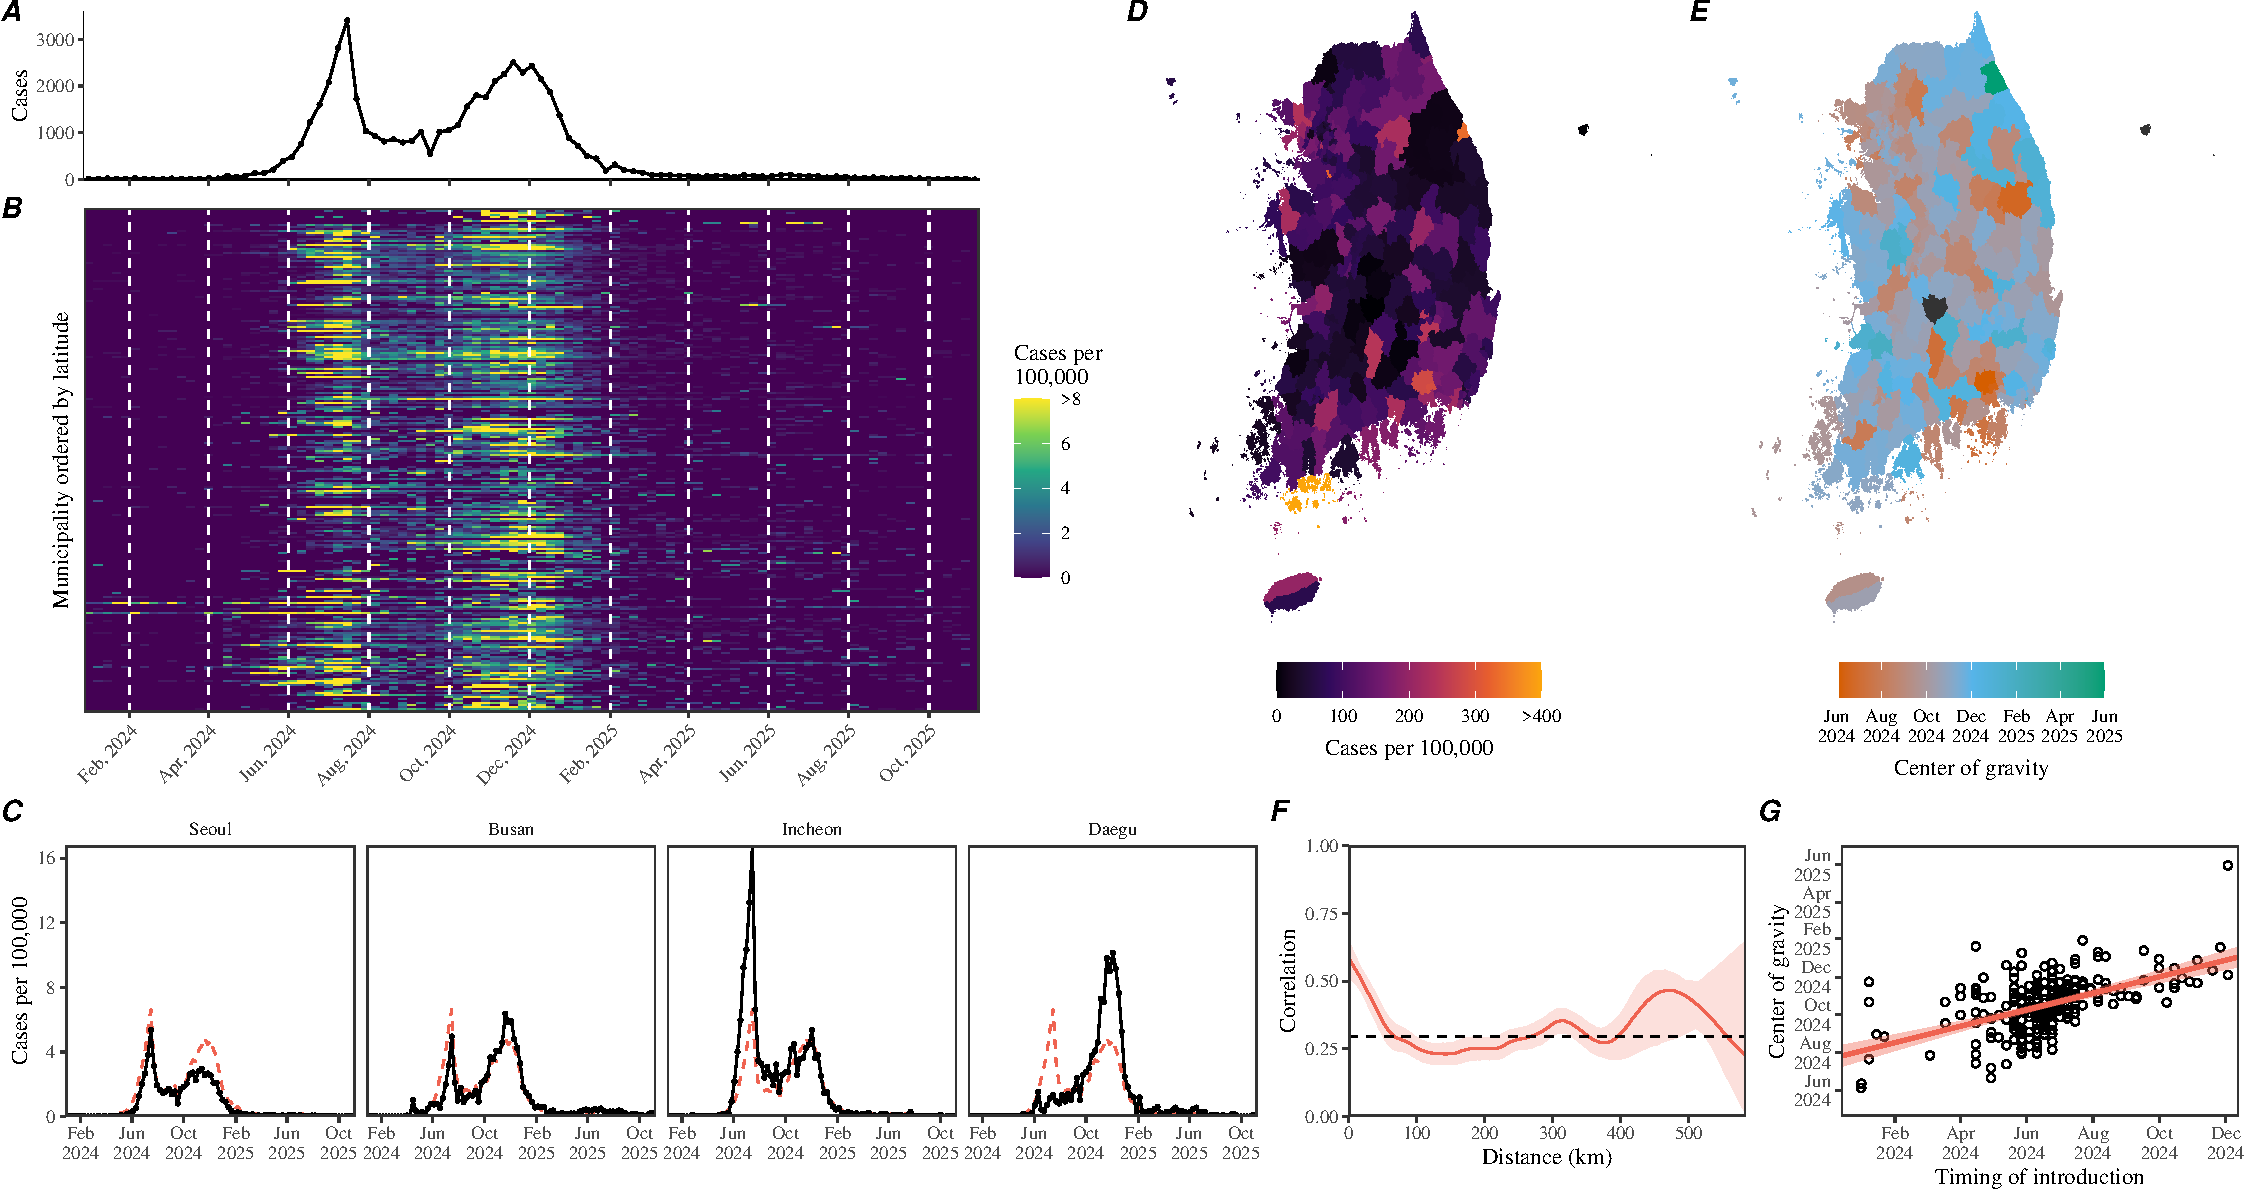
\includegraphics[width=\textwidth]{../figure/figure_data_spatial.pdf}
\caption{
\textbf{Spatiotempordal dynamics of pertussis outbreak in Korea, 2024---2025.}
(A) Total number of reported cases in Korea.
(B) Number of reported cases per 100,000 individuals by municipality, ordered by latitude.
(C) Number of reported cases per 100,000 individuals in four most populated cities in Korea.
(D) Map of pertussis cases per 100,000 individuals between January 2024 and November 2025.
(E) Map of center of gravity, which represents the mean timing of cases.
(F) Spatial synchrony in logged cases as a function of distance.
The red solid line and shaded regions represent the median estimate and the corresponding 95\% confidence interval.
The dashed horizontal line represents the mean correlation.
(G) Relationship between center of gravity and the timing of introduction, defined as the first week when the number of reported cases is greater than 1 in 100,000.
The red solid line and shaded regions represent the linear regression fit and the corresponding 95\% confidence interval.
}
\end{figure}

To address this question, we combine a detailed spatiotemporal surveillance data from 252 municipalities in Korea (Figure 1) with mathematical modeling approaches. 
We begin by showing that asynchrony in pertussis epidemics, captured by heterogeneous epidemic timing, is associated with differences in introduction delays.
In contrast, the analysis of transmission dynamics reveals synchrony in underlying transmission patterns.
Integrating these findings into a mathematical model illustrates that the apparent asynchrony can be explained by differences in initial epidemic conditions (i.e., introduction delays and initial susceptibility).

\subsection*{Asynchrony in pertussis epidemics associated with introduction delays}

First, to characterize spatial heterogeneity in pertussis waves across Korea, we quantify the center of gravity (Figure 1E), which represents the mean timing of cases \citep{pitzer2015environmental}.
Notably, we find a sharp contrast between early (orange) and late (light blue) waves between many neighboring municipalities (Figure 1E), suggesting spatial asynchrony in pertussis dynamics.
To systematically evaluate this apparent asynchrony, we estimated the spatial synchrony function, which captures changes in correlation in epidemic dynamics as a function of distance \citep{grenfell2001travelling}.
The spatial synchrony function confirms a sharp reduction in cross-correlation with distance (Figure 1F).
For example, within 100km of distance, the cross-correlation drops below 0.25.
By comparison, pertussis epidemics in the US maintained cross-correlations above 0.2 even at 1,000 km \citep{choisy2012changing}, highlighting the fine-scale asynchrony in pertussis epidemics in Korea.
Interestingly, the variation in the center of gravity significantly correlates with the introduction timing ($\rho=0.53$; 95\%CI: 0.44---0.62; Figure 1G), suggesting that differences in introduction timing may contribute to the apparent spatial asynchrony.

\subsection*{Synchrony in temporal changes in pertussis transmission}

\begin{figure}[!th]
\includegraphics[width=0.9\textwidth]{../figure/figure_R_t.pdf}
\caption{
\textbf{Spatial variatoin in the estimates of effective reproduction number.}
(A) Each black line represents the estimated effective reproduction number for a given municipality with more than 400 total cases. 
The red solid line and shaded regions represent the median and 95\% quantiles of effective reproduction number estimates.
(B) Relationship between correlation coefficient for $\mathcal R(t)$ and correlation coefficient for reported cases across all pairwise municipality combinations with more than 400 total cases.
(C) Spatial synchrony in $\mathcal R(t)$ (red) versus logged cases (black) as a function of distance.
The solid line and shaded regions represent the median estimate and the corresponding 95\% confidence interval.
The dashed horizontal line represents the mean correlation.
(D) Estimated multiplicative effects on $\mathcal R(t)$ from the regression analysis.
The blue shaded violin represents the distribution of intercept effect, where a separate intercept term is estimated for each municipality.
The red lines represent the estimated susceptible depletion effect for each municipality.
The orange line and shaded regions represent the estimated changes in transmission from a smooth term and the corresponding 95\% confidence interval.
}
\end{figure}

We then ask whether the observed epidemic asynchrony can be explained by the differences in transmission patterns.
To do so, we quantify the effective reproduction number $\mathcal R(t)$, which measures the average number of new infections caused by a single infected individual \citep{wallinga2007generation,cori2013new}.
For this analysis, we focus on municipalities with more than 400 total cases reported because $\mathcal R(t)$ estimates can be unstable when the number of infections are low.

Notably, $\mathcal R(t)$ estimates appear to be largely homogeneous across different regions, despite the apparent heterogeneity in the observed epidemic dynamics (Figure 2A).
Comparisons of correlation coefficients in $\mathcal R(t)$ versus correlation coefficients in reported cases between all pairwise municipality combinations confirm this observation (Figure 2B).
In 830 out of 861 municipality combinations, correlation in $\mathcal R(t)$ is higher than correlation in cases.
This is reflected in the spatial synchrony function for $\mathcal R(t)$ (Figure 2C), where the mean cross-correlation for $\mathcal R(t)$ ($\rho=0.71$) is considerably higher than that for cases ($\rho=0.30$).

\begin{figure}[!ht]
\includegraphics[width=\textwidth]{../figure/figure_stanfit_region.pdf}
\caption{
\textbf{Fine-scale spatiotemporal variation in pertussis epidemic can be explained with a simple SEIR model.}
(A) Comparisons between the observed and predicted epidemic dynamics across municipalities with more than 400 total cases, ordered by latitude..
(B) The bar plot represents the distribution of R squared values for model fits.
The vertical dashed line represents the median.
(C) Relationship between the estimated and predicted center of gravity.
The solid line indicated the one-to-one relationship.
(D) Relationship between the initial susceptible $S(0)$ and infected $I(0)$ fraction with center of gravity.
Points represent the estimates for each municipality.
(E) Impact of initial susceptibility on pertussis epidemic dynamics.
(F) Estimated time-varying pertussis transmission rate.
The red line and shaded regions represent the posterior median and the corresponding 95\% credible interval.
}
\end{figure}

To better understand factors driving changes in $\mathcal R(t)$, we perform a regression analysis using a generalized additive model with three covariates \citep{te2013driving,wood2017generalized,kissler2020projecting}: (1) a municipality-level fixed effect allowing each municipality to have its own intercept; (2) a cumulative-cases term capturing the effect of susceptible depletion; and (3) a single smooth term shared across municipalities, which allows for temporal changes in pertussis transmission over time, such as seasonal forcing.
First, the smooth term suggests a strong transmission reduction around August and February, which coincide with the timing of school breaks (Figure 2D).
Second, the model estimates a significant effect of effect of susceptible depletion (Figure 2D; $p<0.001$).
Notably, this simple regression model explains 84\% of variance in $\mathcal R(t)$, suggesting that the observed temporal fluctuations in transmission can be largely explained by school-related seasonality and the gradual depletion of susceptible individuals.
Taken together, the analysis of center of gravity and $\mathcal R(t)$ suggest that differences in introduction timing and susceptible host dynamics are likely main drivers for spatial asynchrony in pertussis epidemics in Korea, rather than variation in seasonal transmission patterns.

\subsection*{Mathematical modeling of fine-scale spatio-temporal pertussis epidemic}

To test whether variation in introduction timing and susceptible dynamics alone can explain the observed epidemic patterns, we extended a standard susceptible-exposed-infected-removed (SEIR) model \citep{rohani2010contact} to jointly estimated a single, time-varying transmission term, which is shared across all regions.
We also allowed spatial variation in initial susceptible $S(0)$ and infected $I(0)$ fraction as well as the reporting rate $\rho$.
Variation in $S(0)$ captures differences in population-level susceptibility, whereas variation in $I(0)$ effectively captures differences in introduction timing.
For this analysis, we also focus on municipalities with more than 400 total cases.
The model is fitted using a Bayesian inference software rstan with 4 independent chains, each consisting of 8000 iterations \citep{carpenter2017stan}.
The convergence was assessed by ensuring low R-hat, high effective sample size, no divergent transitions, and no iterations that exceeded the maximum tree depth.

Our simple transmission model that assume shared transmission rate can capture fine-scale spatiotemporal variation of pertussis outbreak in Korea (Figure 3A) with a median R squared value of 0.86 (95\% quantile: 0.71---0.91).
Furthermore, we find a near-perfect correlation between the predicted and observed center of gravity (Figure 3C).
So what factors determine the timing of epidemic, and therefore the center of gravity?
We address this question by simulating our model between April 2024 and April 2025 across plausible ranges of $S(0)$ and $I(0)$.

First, increasing $I(0)$ leads to an earlier epidemic because it permits earlier introduction of the infection to the population (Figure 3D).
This is consistent with our earlier observations (Figure 1F).
Similarly, increasing $S(0)$ also results in an earlier epidemic.
This is because high levels of susceptibility allows for a large first wave, which prevents the second wave through the overcompensatory susceptible depletion (Figure 3E).
Finally, we estimate that the large reduction in transmission around late July 2024 and late January 2025 allowed the occurrence of two distinct epidemic waves (Figure 3F).
this estimated timing of transmission reduction is consistent with our estimates from the $\mathcal R(t)$ analysis and coincide with the timing of school holidays in Korea.

We validate our model by taking the estimated transmission term and fitting the remaining parameters (i.e., initial infected, initial susceptible, and reporting probability) to data from the remaining 210 municipalities with less than 400 total cases (Figure S2).
While model predictions appear consistent with the observed patterns (Figure S2A),
we estimate a lower value for the median R squared: 0.58 (95\% quantile: 0.04--0.87; Figure S2B).
Nonetheless, our analysis suggests that the majority of asynchrony in pertussis epidemics can be explained via the differences in introduction timing and initial susceptibility.

\section*{Summary}

Understanding mechanisms that drive spatiotemporal variation in epidemic dynamics is a major aim for infectious disease dynamics and control 
\citep{pitzer2015environmental,dalziel2018urbanization,pons2018seasonality,baker2019epidemic,grenfell2001travelling,cummings2004travelling,viboud2006synchrony}
The large pertussis outbreaks in Korea that occurred between 2024 and 2025 presents a unique perspective on a fine-scale spatiotemporal asynchrony heterogeneity in epidemic dynamics: 
some municipalities experienced two epidemic waves while other places experienced only the first or second without a clear patterns of synchrony.
We propose that this variation can be explained by the differences in introduction delays and initial susceptibility, where high levels of susceptibility can cause a large first wave and prevent the second wave through susceptible depletion.
Incorporating this idea into a simple transmission model by allowing for a joint estimation of a single transmission rate with variation in initial epidemic conditions confirms our hypothesis.
Together, these findings demonstrate that differences in initial epidemic conditions---rather than variation in transmission---can generate fine-scale asynchrony, offering a general framework for understanding the spatiotemporal dynamics of re-emerging infections.

\section*{Caveats and future directions}

Even though our model explains the observed dynamics reasonably well, there are several limitations to our work.
First, our model is purely deterministic and does not account for stochasticity, which is likely an important factor for characterizing the establishment of infections after the initial invasion and the subsequent dynamics, especially in small populations \citep{finkenstadt2002stochastic,lloyd2005superspreading,magpantay2016pertussis}.
Second, we estimated that a variation in susceptibility can explain the observed epidemic patterns, but we were unable to identify the mechanism that explains this variation.
For example, we hypothesized that past vaccine coverage would explain variation in susceptibility given the role of waning immunity in driving pertussis re-emergence \citep{wearing2009estimating,tan2015pertussis,domenech2018impact}, but we did not find a significant correlation (Figure S3).

Our parameter estimates must be interpreted with care as our model relies on several simplifying assumptions.
For example, we assumed the same values of basic reproduction number $\mathcal R_0$ across all municipalities.
Therefore, any regional variation in $\mathcal R_0$, driven by differences in contact rates and age distributions would be captured in our estimate of the initial susceptible fraction.
In other words, our estimated susceptible fraction should be interpreted as the effective susceptibility that also captures behavioral and sociological factors, beyond immunological differences.
We also did not consider an age structure in our model, but age-structured contact patterns play an important role in shaping pertussis transmission \citep{rohani2010contact}.
For example, \cite{cho2024pertussis} recently suggested transmission among elderly may contributed to the persistence of pertussis in Korea.
Despite these limitations, our work provides a quantitative foundation and empirical evidence for understanding epidemic asynchrony.

\section*{Conclusion}

The continued emergence of new pathogens and re-emergence of vaccine preventable infections, such as pertussis, highlights the importance of identifying hotspots of future outbreaks and developing targeted intervention strategies \citep{heymann2001hot,naguib2020towards,nguyen2022enterovirus}.
The apparent asynchrony in pertussis epidemic in Korea, driven by the differences in introduction timing and population-level susceptibility, underlines the importance of detailed pathogen surveillance for early detection and strategic allocation of prevention and control resources..
Immunological surveillance platforms will be particularly useful for evaluating potential risk of pathogen re-emergence in the future \citep{mina2020global,nguyen2025dynamics}.
A detailed understanding of spatial variation in population-level immunity will be crucial for predicting spatiotemporal dynamics of future outbreaks.

\bibliography{whooping-cough}

\end{document}
